\section{Diagrams}


Here we keep all the diagrams.
They belong to the $D$ language in the introduction (\S\ref{sec:intro})
and need updating to cover $P$.

\subsection{atomic-action}
\includegraphics{images/atomic-action}

\subsection{conditional-actual}
\includegraphics{images/conditional-actual}

\subsection{iteration-actual}
\includegraphics{images/iteration-actual}

\subsection{par-comp-actual}
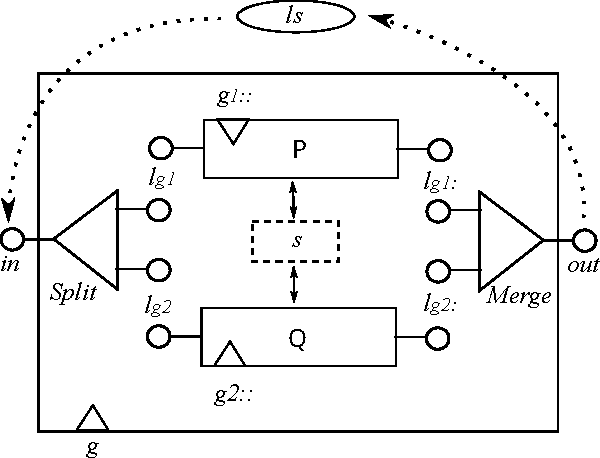
\includegraphics{images/par-comp-actual}

\subsection{seq-comp-actual}
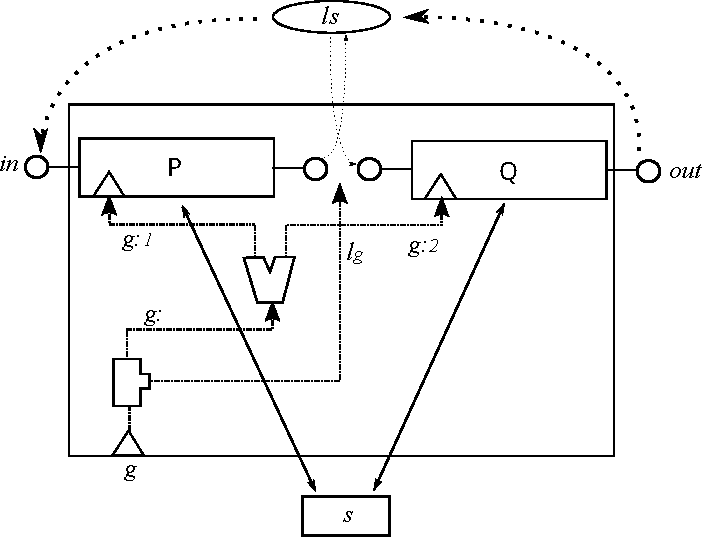
\includegraphics{images/seq-comp-actual}

\subsection{label-gen-example}
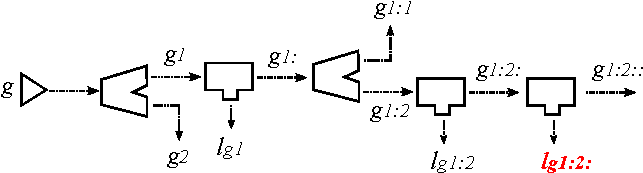
\includegraphics{images/label-gen-example}

\subsection{parallel-label-gen}
\includegraphics{images/parallel-label-gen}

\subsection{split-gen}
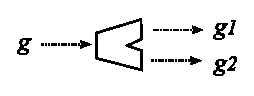
\includegraphics{images/split-gen}

\subsection{parallel-program}
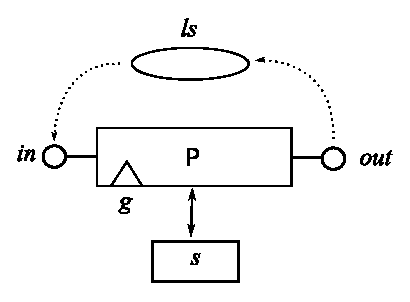
\includegraphics{images/parallel-program}

\subsection{seq-comp-idea}
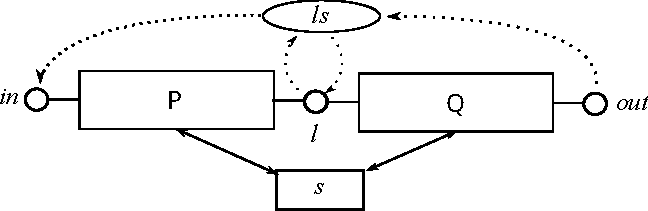
\includegraphics{images/seq-comp-idea}

\subsection{new-label}
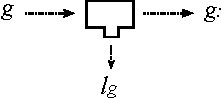
\includegraphics{images/new-label}
